% !TEX TS-program = xelatex
% !TEX encoding = UTF-8 Unicode
% !Mode:: "TeX:UTF-8"

%This file contains the LaTeX code of my laboratory report for my ICS II course.
%Author: 张作柏/Zuobai Zhang <17300240035@fudan.edu.cn>

% This is a simple template for a LaTeX document using the "article" class.
% See "book", "report", "letter" for other types of document.

\documentclass[12pt]{article} % use larger type; default would be 10pt

\usepackage[utf8]{inputenc} % set input encoding (not needed with XeLaTeX)

%%% Examples of Article customizations
% These packages are optional, depending whether you want the features they provide.
% See the LaTeX Companion or other references for full information.

%%% PAGE DIMENSIONS
\usepackage[top=1.05in, bottom=0.95in, left=0.90in, right=0.95in]{geometry}
%\usepackage{geometry} % to change the page dimensions
\geometry{a4paper} % or letterpaper (US) or a5paper or....
% \geometry{margin=2in} % for example, change the margins to 2 inches all round
% \geometry{landscape} % set up the page for landscape
%   read geometry.pdf for detailed page layout information

\usepackage{graphicx} % support the \includegraphics command and options

% \usepackage[parfill]{parskip} % Activate to begin paragraphs with an empty line rather than an indent

%%% PACKAGES
\usepackage{booktabs} % for much better looking tables
\usepackage{array} % for better arrays (eg matrices) in maths
\usepackage{paralist} % very flexible & customisable lists (eg. enumerate/itemize, etc.)
\usepackage{verbatim} % adds environment for commenting out blocks of text & for better verbatim
\usepackage{subfigure} % make it possible to include more than one captioned figure/table in a single float
% These packages are all incorporated in the memoir class to one degree or another...

%%% HEADERS & FOOTERS
\usepackage{fancyhdr} % This should be set AFTER setting up the page geometry
\pagestyle{fancy} % options: empty , plain , fancy
%\renewcommand{\headrulewidth}{0pt} % customise the layout...
\lhead{}\chead{}\rhead{}
\lfoot{}\cfoot{\thepage}\rfoot{}

%%% SECTION TITLE APPEARANCE
\usepackage{sectsty}
\allsectionsfont{\sffamily\mdseries\upshape} % (See the fntguide.pdf for font help)
% (This matches ConTeXt defaults)

%%% ToC (table of contents) APPEARANCE
\usepackage[nottoc,notlof,notlot]{tocbibind} % Put the bibliography in the ToC
\usepackage[titles,subfigure]{tocloft} % Alter the style of the Table of Contents
\renewcommand{\cftsecfont}{\rmfamily\mdseries\upshape}
\renewcommand{\cftsecpagefont}{\rmfamily\mdseries\upshape} % No bold!
\usepackage{titletoc}
\titlecontents{section}
              [1.5cm]
              {\bf \large}%
              {\contentslabel{1.8em}}%
              {}%
              {\titlerule*[0.5pc]{$\cdot$}\contentspage\hspace*{0.6cm}}%
		   [\vspace{0.5em}]
\titlecontents{subsection}
              [1.8cm]
              {\normalsize}%
              {\contentslabel{2.0em}}%
              {}%
              {\titlerule*[0.5pc]{$\cdot$}\contentspage\hspace*{0.6cm}}%
		   [\vspace{0.4em}]
\titlecontents{subsubsection}
              [2.1cm]
              {\small}%
              {\contentslabel{2.5em}}%
              {}%
              {\titlerule*[0.5pc]{$\cdot$}\contentspage\hspace*{0.6cm}}%
		   [\vspace{0.4em}]
		  


\usepackage[UTF8]{ctex}
\usepackage{fancyhdr}
\usepackage{enumerate}
\usepackage{indentfirst}
\usepackage{extramarks}
\usepackage{titling}
\usepackage{xcolor}
\usepackage{fontspec}
\usepackage[CJKbookmarks=true,colorlinks,linkcolor=black]{hyperref}
\setmainfont{Times New Roman}

\usepackage{etoolbox}
\makeatletter
\providecommand{\subtitle}[1]{% add subtitle to \maketitle
	\apptocmd{\@title}{\par {\large #1 \par}}{}{}
}
\makeatother

%%% END Article customizations

%%% The "real" document content comes below...

%\title{\textbf{Digital Logic and Computer Design Report}}
\title{\textbf{捧哏生成器与人物对话机}}
\subtitle{——对话系统的两种应用实践}
\author{张作柏\\17300240035}
%\date{} % Activate to display a given date or no date (if empty),
         % otherwise the current date is printed 

\usepackage{amsmath}
\usepackage{ulem}


\begin{document}
\begin{sloppypar}
\maketitle

\pagestyle{fancy}
\lhead{\textbf{{\thetitle}}}
\rhead{\textbf{\nouppercase{\firstleftmark}}}
\cfoot{\thepage}

\thispagestyle{empty}
\tableofcontents
\clearpage

\setcounter{page}{1}


\section{引言:对话系统之三生三世}

实现高度智能的人机对话系统,一直以来都是自然语言处理领域高度关注的课题之一。近年来,随着深度学习技术的广泛应用,聊天机器人的智能性得到了很大幅度的提升。一方面,随着互联网的普及,可获取的数据量大大增加,这为我们构造数据驱动的对话系统提供了便利。另一方面,深度学习方法能够有效地捕获大数据中暗含的规律,在计算机视觉、自然语言处理、推荐系统等领域中都有广泛地应用。因此,探究深度学习方法在构建对话系统中的应用是目前主要的研究趋势。

根据综述~\cite{chen2017survey}中的定义,可将对话系统按目的分为两类:(1){\bf 任务驱动型}与(2){\bf 非任务驱动型},或称聊天机器人。任务驱动型系统旨在借助聊天功能帮助用户完成一定的功能,例如,寻找商品,预定酒店,疑难解答等。而非任务驱动型系统的目的则是与用户进行不限话题的闲聊,更多是用于娱乐,比如微软小冰,QQ小冰等聊天机器人。本项目主要关注后者,即非任务驱动型的对话系统设计。

如前所述,对于闲聊型的聊天机器人,目前仍缺少合适的应用场景。本项目中,我们成功地将闲聊系统的思想用在了两个不同的场景中:{\bf 相声中捧哏的生成}与{\bf 人格化的对话机器人}\footnote{最初仅实现了人格化聊天,但是自己对实现效果并不满意,恰好又有了捧哏生成器的想法,于是就在截止日期前几天又完成了第一个应用的设计。}。
\vspace*{-0.25cm}
\begin{itemize}
\item 相声是起源于中国华北地区的一种民间曲艺,其主要表演形式为多人之间对话。双口相声中常分逗哏与捧哏两角,捧哏主要负责配合逗哏叙述故事情节。相声中对话的表演形式与对话系统的技术可以非常自然地相结合,{\bf 本项目中我们依照构建对话系统的方法实现了一个简单的捧哏生成器}\footnote{项目代码开源于\url{https://github.com/Oxer11/Crosstalk-Generation}}。\vspace*{-0.3cm}
\item 受性别、性格、年龄等因素影响,不同人之间的说话风格迥异。每个人都有自己独特的说话风格,比如惯用语、方言等等。或许你曾想过对话丘吉尔、托尔斯泰等大文豪,亦或是与自己的爱豆来一次亲切的交流,{\bf 本项目中我们以《星球大战》系列电影中的经典角色卢克·天行者为例,对如何融合个性化因素到对话系统中,进行了一些简单地尝试}\footnote{项目代码开源于\url{https://github.com/Oxer11/Chat-with-Skywalker}}。
\end{itemize}

\subsection{相关工作}

实现聊天机器人常见的方法有{\bf 生成类模型}与{\bf 检索类模型}。生成类模型可以生成更恰当的回复,且可以生成不在语料库中的回复;而检索类模型则可以保证回复的流畅程度与所包含的信息量~\cite{ji2014information}。

对于生成类模型,最常见的方法是将对话的生成视为机器翻译的过程。~\cite{ritter2011data}中提出了一种基于统计机器翻译的生成模型~\cite{zens2002phrase}。因深度学习在机器翻译中的出色表现,自然也会联想到将深度学习用于对话生成中。其中,最著名的框架当属Sutskever等人在2014年提出的seq2seq模型~\cite{sutskever2014sequence},Vinyals等人于2015年首次将seq2seq模型用于对话生成这一任务中~\cite{vinyals2015neural},实现了较大的性能提升。但生成类模型会受到两类问题的影响:
\begin{enumerate}
	\item 模型倾向于生成无意义的回答,例如“I don't know.”为了解决这类问题,李纪为等人提出了使用最大互信息(MMI)作为目标函数的训练方法~\cite{li2016diversity},起到了一定的提升。往后仍有许多后继工作~\cite{shao2017generating}在研究如何生成多样的、有意义的回复。\vspace*{-0.2cm}
	\item 模型不能保证回复的一致性,常出现前后回答不一致的情况,例如对于“Where are you from?”和“Where do you come from?”两问题分别回答“The US”和“London”,这就出现了不一致。为解决这一问题,李纪为等人提出了用特征向量描述人这一个体,使其回答前后一致的方法~\cite{li2016persona}。而后续仍有许多工作~\cite{zhang2018personalizing,su2019personalized}研究如何通过不同的数据集来构造前后一致的个性化聊天机器人。
\end{enumerate}

对于检索类模型,常见的方法是使用匹配的模式,~\cite{lu2013deep}中提出了一种基于深度神经网络的短文本选择匹配模型,~\cite{hu2014convolutional}使用卷积神经网络提升了这一方法的性能。

本项目中,我们先使用最基本的seq2seq模型搭建了一个简单的生成式模型,能够完成简单的日常对话。对于相声捧哏的生成,我们直接将该模型应用于相声数据集上以检验其性能。而对于人格化的聊天机器人,简单的生成模型无法非常好的捕获个人的说话风格,所以我们则使用检索类模型。

%\newpage
\vspace*{-0.4cm}
\section{基本模型:对话系统架构之魂}

\subsection{模型架构}

\subsubsection{seq2seq框架}

将seq2seq框架应用于对话生成的想法最早由Vinyals等人提出~\cite{vinyals2015neural},其直接思想是将对话生成看做机器翻译问题。seq2seq属于encoder-decoder结构的一种,基本思想是利用两个RNN,分别作为encoder和decoder。

\begin{figure}[h]
	\centering
	\includegraphics[width=0.8\linewidth]{figure/seq2seq.png}
	\caption{seq2seq框架示意图\protect\footnotemark}
	\label{fig:seq2seq}
\end{figure}
\footnotetext{图源\url{https://gitee.com/zyfeng_nlp/Seq2Seq-PyTorch}}

\paragraph{{\bf Encoder}} encoder将输入序列压缩为指定长度的向量,这个向量就可以看成是这个序列的语义,此过程称为编码。或者将输入序列的所有隐藏状态通过变换得到语义变量。我们的模型中使用的是GRU~\cite{chung2014empirical}来实现RNN,以避免梯度爆炸、梯度消失等问题。

\paragraph{{\bf Decoder}} decoder负责根据语义向量生成指定的序列,这个过程也称为解码。如图~\ref{fig:seq2seq}所示,我们将encoder得到的编码向量作为decoder的输入向量,每轮根据当前RNN的输出状态对当前词进行预测,并将预测词作为下一次的输入。



\subsubsection{Attention机制}

Attention机制最早由Google DeepMind团队在2014年提出~\cite{mnih2014recurrent},而后Bahdanau等人将该机制应用于机器翻译任务中~\cite{bahdanau2014neural}。Attention机制可直观理解为我们的视觉在感知物体时,不会从头到尾每次都看,而是根据需求关注特定的一部分。而注意力这一机制可以通过为不同位置分配不同权值来实现。由于这一机制并不是本项目的重点,故在此不展开解释其原理,具体实现可参考原论文~\cite{bahdanau2014neural}与代码教程\footnote{\url{https://github.com/spro/practical-pytorch/blob/master/seq2seq-translation/seq2seq-translation-batched.ipynb}}。

\begin{figure}[h]
	\centering
	\includegraphics[width=0.8\linewidth]{figure/attention.png}
	\caption{Attention机制示意图\protect\footnotemark}
\end{figure}
\footnotetext{图源\url{https://gitee.com/zyfeng_nlp/Seq2Seq-PyTorch}}

\subsubsection{个体特征向量}

为了保证对话回复的上下文一致性,李纪为等人提出了引入个体特征向量的方法~\cite{li2016persona}。该方法的思路为,对每个对话者创建一个embedding向量,用于编码其特征。在decoder进行回复生成时,将对话者的embedding向量和上一位的预测单词作为每个单元的输入。这一方法被证明有效地改善了回答的上下文一致性,并能较好的融入对话者的个人信息。

\subsection{代码实现}

代码实现共两个版本:第一个版本用seq2seq的框架结合个体特征向量实现了一个简单的对话生成模型。该版本只实现了CPU的版本,仅可用于演示模型效果。具体实现可见test.ipynb文件,其中演示了模型在小数据集上过拟合的情况(正确实现的模型应能过拟合小数据集)。第二个版本直接使用了开源的代码\footnote{\url{https://github.com/ywk991112/pytorch-chatbot}},其中使用的是seq2seq框架并引入了attention机制,因其实现接口清晰,便于使用,故后续实验均使用第二个版本\footnote{在调试版本一的过程中听闻可以使用开源代码,于是找到了版本二,故版本一仅用作展示。}。

\subsection{数据集选择}

\paragraph{{\bf Cornell Movie--Dialogs Corpus}~\cite{Danescu-Niculescu-Mizil+Lee:11a}} 该语料库包含了从电影片段中直接抽取出的对话,对话的元数据比较详实。其中包含了10,292对电影角色之间的220,579次对话交流,总共9,035名角色来自617部电影,总共304,713次说话。语料库提供的元数据包含电影的体裁、上映年份、IMDB评分、IMDB评价次数、角色性别、在电影中的分量。\\
{\bf 注1:} 因为论文发表于2011年,所以只包含了2011年之前的电影,导致很多近几年的电影未包含其中。\sout{有不少自己喜欢的电影未在其中。}\\
{\bf 注2:} 由于对话是直接从电影中提取的,所以比较粗糙,不一定符合日常对话的习惯。

\paragraph{{\bf OpenSubtitles}~\cite{tiedemann2009news}} 该语料库包含了从字幕网站收集的电影对话。语料库包含了约60M到70M的电影对话,更大更粗糙,但是未提供数据的元信息,即不知道每段对话是出自于哪部电影的哪对角色。

\paragraph{{\bf DailyDialog}~\cite{li2017dailydialog}} 该数据集包含了日常生活中可能出现的对话,是由人手工书写的,质量较高。其对话均是在某个具体场景下发生的,因此更加关注于某个具体的话题,比如售货员与顾客之间的对话。该语料库总共包含13,118次对话,平均每次对话7.9轮。

\subsection{模型训练}

对于Cornell Movie Dialogs Corpus,我们在test.ipynb演示了版本一模型在小数据集上过拟合的情形。对于整个语料库,我们使用单层双向GRU网络作为encoder,隐状态分别设置为256、512进行训练,最终模型收敛,但是效果并不理想。

对于OpenSubtitles语料库,我们同样使用单层双向GRU网络作为encoder,隐状态分别设置为256、512进行训练。但是,训练两周后Perplexity仍停留在1000左右,故选择放弃该语料库。

对于DailyDialog语料库,我们使用双层双向GRU网络作为encoder,隐状态设置为256,训练两天后模型收敛,效果比较好,很大程度上可能是因为其数据质量较高。

最终选择DailyDialog语料库上训练所得模型作为后续工作的基础模型。其余模型训练失败的原因会在第\ref{sec:error}节进行详细分析。

\subsection{效果演示}

\begin{figure}[h]
	\centering
	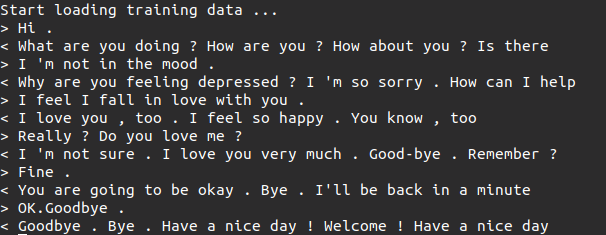
\includegraphics[width=0.9\linewidth]{figure/conv1.png}
	\caption{对话效果}
	\label{fig:conv}
\end{figure}

图~\ref{fig:conv}演示了一段简单(\sout{精挑细选过})的人机之间的对话,其模型来自于DailyDialog训练结束后得到的模型。可以发现,单句对话基本已能产生比较合理的回复,虽然上下文仍缺少联系。值得注意的一点是,我的聊天机器人倾向于产生比较长的回答,且有的回答仍不完全符合逻辑,比如说过Goodbye后紧接着又说Welcome。这一点可能是因为数据集太小,模型泛化性能不佳。

%\newpage
\section{捧哏生成器:和于谦老师说段相声}

\subsection{任务简介}

相声(Crosstalk)是一种民间说唱曲艺,它以说、学、逗、唱为形式,突出其特点。其中双口相声指由逗哏、捧哏两个演员对讲的相声。逗哏,是指双口相声演出时不断地说出笑料以让人发笑的主要叙述故事情节的演员,即相声中的“主角”。而逗哏则是双口相声演出时配合逗哏叙述故事情节的演员。双口相声中,通过捧逗的衬托、铺垫,逗哏与捧哏合作,使叙述中逐渐组成包袱,产生笑料。

俗话说,“三分逗,七分捧”,别看捧哏说话简单,却是个技术活。捧哏的技巧体现在捧哏的时机、所做的动作及其所使用的话语,不恰当的话语使用反而会使观众一头雾水。本项目旨在设计一个捧哏生成器,\sout{训练出一个人工智能界的于谦大爷}。

\subsection{数据收集与预处理}

数据集使用的是在Github上的开源的相声数据集\footnote{\url{https://github.com/unarxiv/crosstalk-dataset}},该数据集是通过爬虫从网上爬取了近一百个相关文本,进行筛选处理后,得到的五十段郭德纲于谦对口相声。我自己也手动搜集了五十段对口相声,可以在data文件夹中找到。但考虑到数据比较脏,且与郭于的相声风格不符,故最终未用于训练(\sout{其实是在自己搜集完后才发现有现成的数据集的})。


\begin{figure}[h]
	\centering
	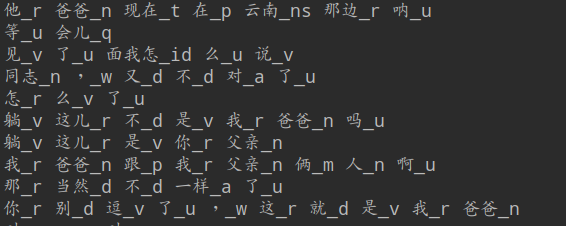
\includegraphics[width=0.9\linewidth]{figure/seg.png}
	\caption{分词效果}
	\label{fig:seg}
\end{figure}

为便于分析捧哏的语言特点,我使用了thulac中文分词工具~\cite{thulac}对句子进行分词,其演示效果如图~\ref{fig:seg}所示。

\subsection{语言特点分析}


\begin{figure}[h]
	\centering
	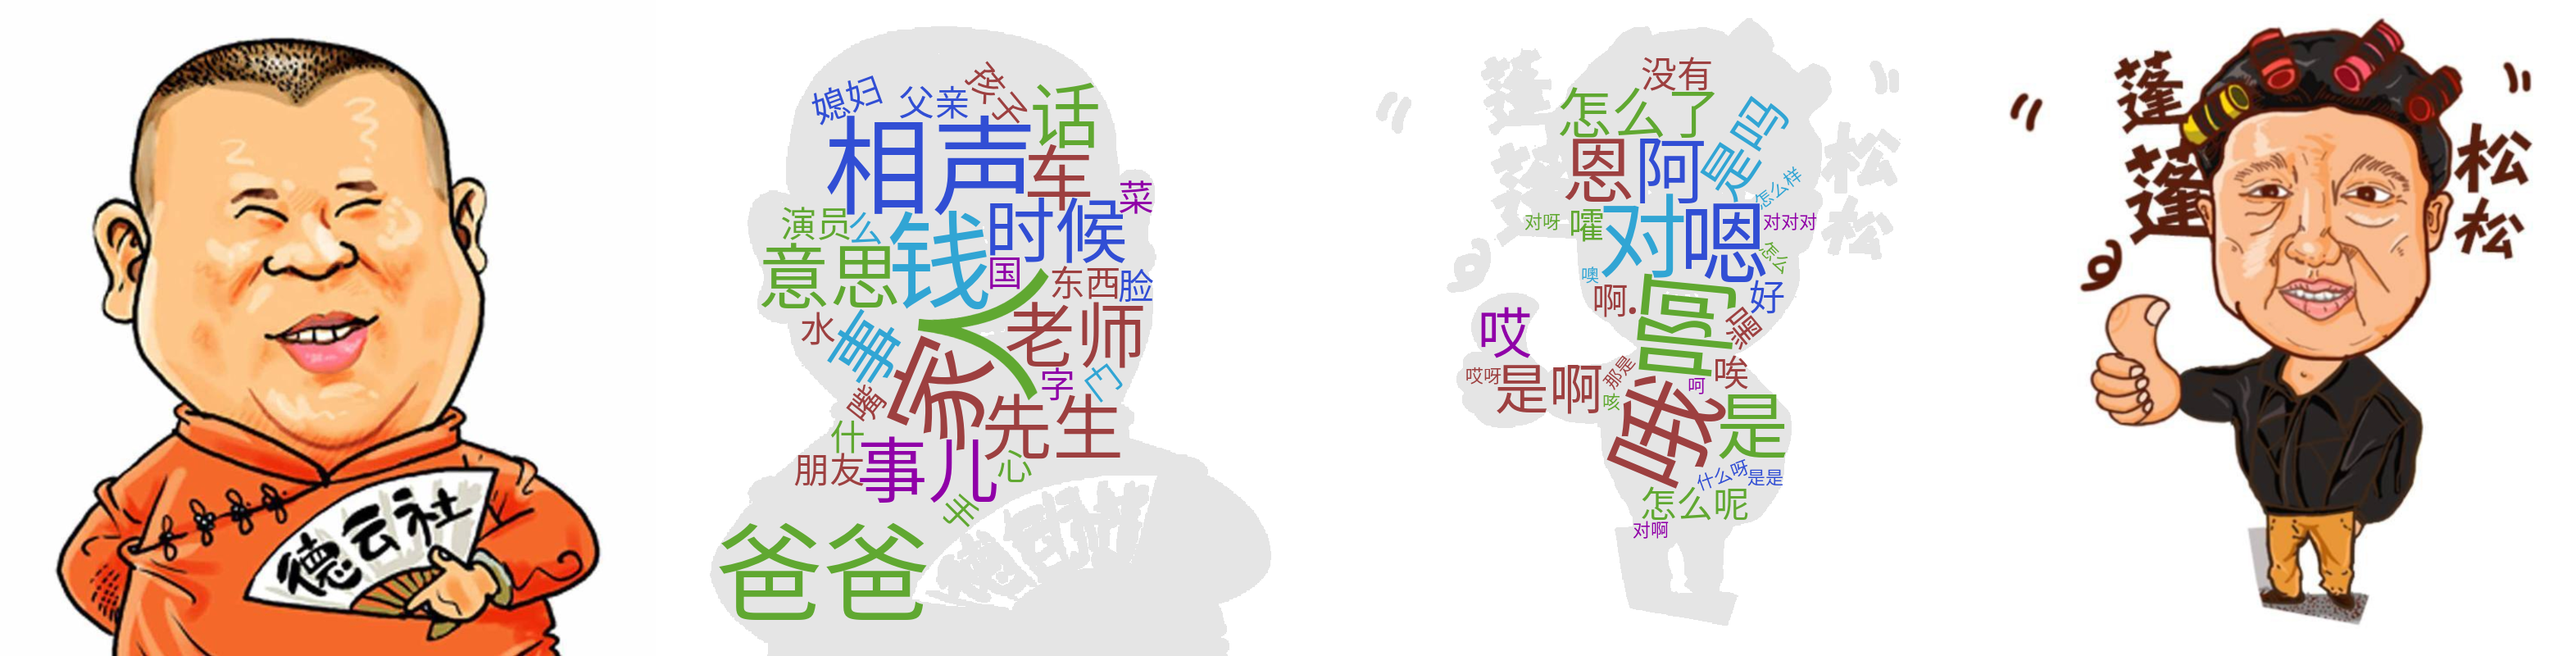
\includegraphics[width=\linewidth]{figure/gy_wc.png}
	\caption{高频词词云图\protect\footnotemark}
	\label{fig:wordcloud}
\end{figure}
\footnotetext{卡通图片源自\url{http://j.17qq.com/article/qssnqwmny.html}}

我们统计了在这50段相声中所有词语的出现频率。对于逗哏,我们统计了所有名词的出现次数,并制作词云图,如图~\ref{fig:wordcloud}左侧所示。出现次数最多的几个词分别是人(806次)、家(497次)、钱(247次)、相声(178次)、爸爸(155次)、老师(113次)。所有的高频名词都是比较{\bf 朴素}、{\bf 口语化}的词,比如意思、媳妇等,其中还有特色的北京{\bf 儿化音}“事儿”等等,非常符合相声的特点。{\bf 值得注意的是,“爸爸”一词出现的频率相当高,这也与郭于相声中于谦老师的父亲经常被“问候”相符。}

对于捧哏,因其话语比较简单,故我们直接统计了所有句子的出现频率,词云图如图~\ref{fig:wordcloud}右侧所示。出现频率最高的几个词分别是啊(281次)、哦(280次)、对(246次)、嗯(211次)、是(150次)。容易发现,捧哏使用的回答确实十分简单,以语气词居多。

\begin{figure}[h]
	\centering
	\subfigure[人名]{
		\begin{minipage}[t]{0.4\linewidth}
			\centering
			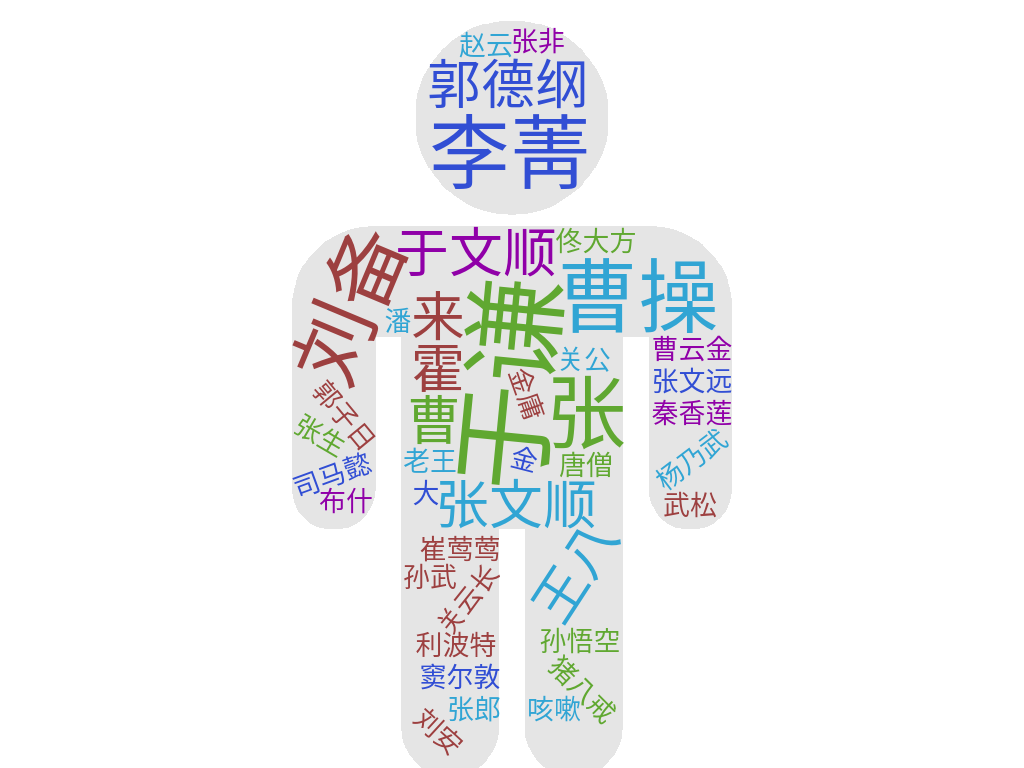
\includegraphics[width=\linewidth]{figure/name_wc.png}
		\end{minipage}%
	}%
	\subfigure[地点]{
		\begin{minipage}[t]{0.4\linewidth}
			\centering
			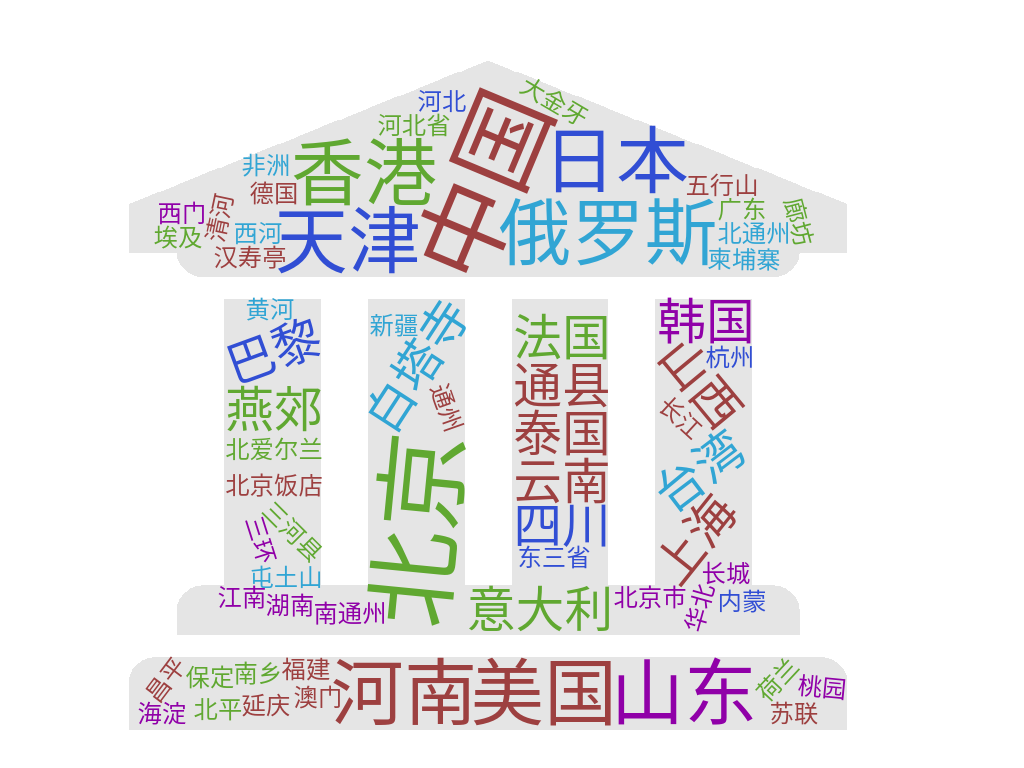
\includegraphics[width=\linewidth]{figure/loc_wc.png}
		\end{minipage}%
	}
	\centering
	\caption{词云图}
	\label{fig:wc}
\end{figure}

除此之外,我们还统计了捧哏中人名与地点的出现次数,其词云图如图~\ref{fig:wc}所示。不出所料,于谦老师霸占了人名榜首,\sout{果然郭于是真爱呀}!同时,还有一些刘备、曹操、关羽等出现频率较高的词,这与相声中时常引用名著典故有关。最常提及的几个地名分别是北京、中国、俄罗斯、美国、山东、河北等,一个现象是其中北方的地名出现频率往往更多,这与相声主要在北方流传密切相关。

\subsection{模型训练}

训练时,我们使用双层的双向GRU网络作为encoder,隐状态大小设置为256,设置batch size为64,训练10000个batch。设置learning rate为0.0001,使用Adam算法进行优化。平均每个batch需要花费7s,训练时长约19个小时,即得到模型。最后模型可完全拟合数据集,每训练1000个batch便保存了一次模型,因此可以选择最合适的模型来进行最终测试。

\subsection{实验结果}

我们使用最终得到的模型进行了一段简单地捧哏生成,如下图所示。逗哏部分是由我自己编造的,捧哏部分则是由捧哏生成器生成的。可以发现,捧哏的语法虽然仍有错误,但是语义已经能比较好的理解,并进行相应的回复了。值得注意的是,{\bf 当逗哏的话中带有儿子时,捧哏可以回复爸爸,说明其已经能够对语义进行一定的理解}。但是,语法上还是有不少错误,比如第一句中的重复,第二句中话未说完就结束,等等。

\fbox{
	\parbox{0.7\linewidth}{
			{\bf 逗:} 今天给大家说段相声。\\
			{\bf 捧:} 怎么样?您给说说啦?怎么样? \\
			{\bf 逗:} 这位我是儿子,于谦。\\
			{\bf 捧:} 你是我爸爸怎么说?我知道你。谁说话是 \\
			{\bf 逗:} 非常高兴跟于老师同台演出。\\
			{\bf 捧:} 哎呀,行了行了行了。 \\
			{\bf 逗:} 捧您是应该的。\\
			{\bf 捧:} 上家去,代言也不能脸上这个?!
	}
}

\vspace{0.5cm}

{\bf 于谦老师的捧哏技巧没学到,暴脾气倒是先学来了...}

出于好奇,我还用这个捧哏生成器为前阵子比较火的说唱歌曲《大碗宽面》捧了个哏,效果如下所示。好吧,好像这里配的有点前言不搭后语,吃错药的状态。

\vspace{0.5cm}

\fbox{
	\parbox{0.7\linewidth}{
		{\bf 逗:} 你看这碗又大又圆\\
		{\bf 捧:} 嗨,呵(长套子)啊\~{}吧\~{}吧\~{}\\
		{\bf 逗:} 你看这面又长又宽\\
		{\bf 捧:} 嘿,好嘛   又 多 大 鼓唱 的 干 嘛 呀 ? \\
		{\bf 逗:} 有时生活特别累\\
		{\bf 捧:} 这 不 是 什 么 意思 呢 。 你 捧 我 送 这 一 句 \\
		{\bf 逗:} 这碗大!\\
		{\bf 捧:} 好 吗 , 拿 一 敲 这个 , 好 吗 , 又 多 一百 炸\\
		{\bf 逗:} 这大碗宽面也很贵\\
		{\bf 捧:} 阿 ? 好 嘛 , 哪 年代 的 事儿 了 ? ? ! 您 这
	}
}


\subsection{思考与改进方向}

总体来看,最后的效果还算可以接受,模型已经能进行简单地语义理解,尽管语法上仍有不完美之处,这可能是因为训练数据集太小的缘故。自我反思后,觉得这个项目还有很大的提升空间,具体体现在以下几点:
\begin{itemize}
	\item {\bf 数据。} 数据集确实是太小了,只有五十段相声,学不到太多知识,且还有许多生词。而且数据清洗的不够彻底,比如很多表示动作、神态的词没有去掉,以及很多错别字没有修正(比如“嗯”和“恩”)。
	\item {\bf 模型。} 现在使用的模型是最简单的seq2seq加attention机制,跟基本的机器翻译或文本生成问题并无太大差异,实际上目前已经有非常多性能更好的开源对话系统模型可供使用,只是最后时间比较急没有去找。
\end{itemize}

%\newpage
\section{人格化对话系统:对话卢克·天行者}

\subsection{任务简介}

你是否有想象过与自己的偶像来一次亲切的交谈,亦或是与书中或电影中的人物面对面的交流,而又或是思念过世的亲人,想再次与其交谈?生活中,我们常有听话识人的本领,这多是因为不同人的说话风格迥异,有自己独特的惯用语。本项目中,我们旨在开发一个能够模仿人的说话口吻的聊天机器人,融合个性化的元素在其中。

在本项目中,我们以《星球大战》系列电影中的经典角色卢克·天行者为例\footnote{其实我自己不是星战粉,本想找Jack Sparrow和Bruce Wayne的台词,但是其系列电影上映较晚,并未包含在电影语料库中。},制作了一款能够模仿其说话风格的聊天机器人。

\subsection{数据处理}

为获取卢克·天行者的台词,我们从Cornell Movie--Dialogs Corpus~\cite{Danescu-Niculescu-Mizil+Lee:11a}中提取了星战相关电影中卢克的台词,存放在Luke.txt文件中,其中包含了星战三部曲中的卢克的232句台词。

\begin{figure}[h]
	\centering
	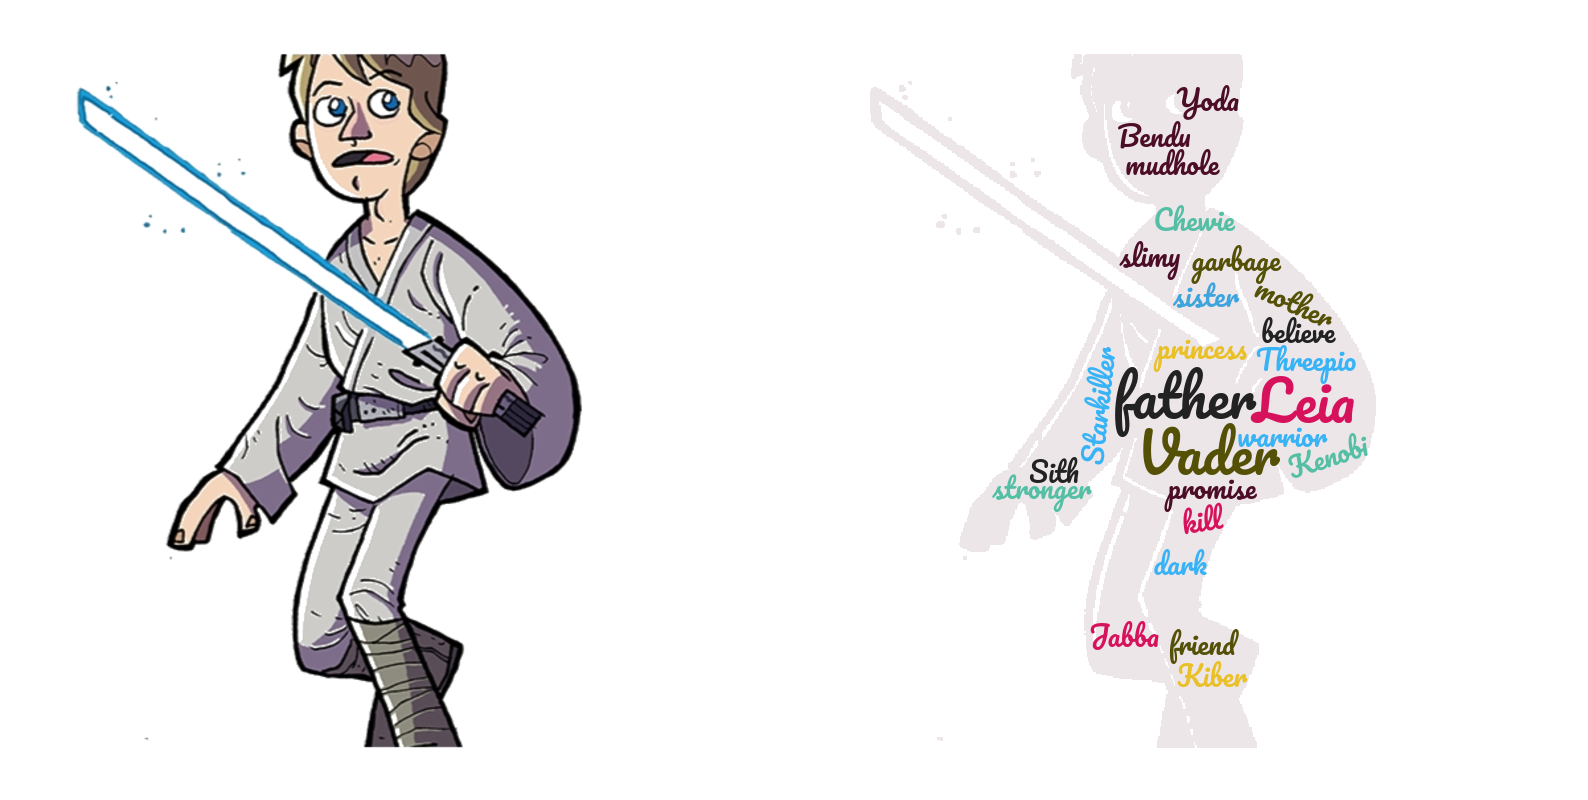
\includegraphics[width=0.9\linewidth]{figure/luke_wc1.png}
	\caption{卢克词云图\protect\footnotemark}
	\label{fig:luke}
\end{figure}
\footnotetext{卡通图片源自\url{https://www.pinclipart.com/pindetail/ThhbTi_star-wars-luke-skywalker-cartoon-clipart/}}

我们也制作了卢克台词的词云图,如图~\ref{fig:luke}所示,可以看到其高频词中包含了Leia、Vader、father等词,非常符合星战系列的故事情节。

\subsection{方法}

在第二节中我们构建了一个基本的对话系统模型,那么如何将卢克的说话方式融合到这一系统中呢?我想到了三种方法:
\begin{enumerate}
	\item {\bf 基于生成的方法。}李纪为等人在~\cite{li2016persona}中提出可将角色embedding为一个特征向量,在decoder生成回答时作为输入,这样产生的回答可以包含角色自身的信息。但是,这种方法在本项目中并不合适,原因有二:1.数据量不足。关于卢克的对话仅有几百组,很难依此生成合乎语法又带有个人风格的回答。2.模型使用背景不符。原文中使用角色特征向量旨在生成上下文一致的回复,而仅一个特征向量很难捕捉卢克的惯用语、高频词的说话习惯。
	\item {\bf 基于分类检索的方法。}可将卢克的所有台词按主题聚类,同时将每个询问分到恰当的类别中,然后再从聚类中挑选合适的台词作为回答。这种方法看似可行,但问题在于缺少合适的聚类方法,以及缺少训练数据,将询问分类需要人工进行,需要消耗大量时间和人力,不可行。
	\item {\bf 基于匹配检索的方法。}先按生成的方法生成一个简单的回答,而后根据语义在卢克的台词库中匹配语义最相近的回答。然而,如何选取判别语义相似性的指标是一个令人头疼的问题。在机器翻译任务中,最常用的指标为BLEU分数~\cite{papineni2002bleu},其原理是计算n-gram的重叠率有多高,但在此问题中使用显然是不合适的。
\end{enumerate}

可以看到这三种方法均有其不合理之处,最终我选择了比较容易实现的第三种方法。其中BLEU分数的计算原理可以参考这篇文章\footnote{\url{https://cloud.tencent.com/developer/article/1042161}},在此不具体讨论。每当生成一个回答后,与语料库中所有的句子计算BLEU分数,取最高的一个句子作为最终回答。我使用的是nltk中提供的计算BLEU分数的函数,并选取unigram和bigram的权重均为0.5,其余均为0。这样选择是因为,n-gram的重叠率实在太低,会导致所有句子的得分都很低,所以只好取n比较小的情况。

\subsection{实验结果}

\fbox{
	\parbox{0.7\linewidth}{
		{\bf Me:} What are you doing?\\
		{\bf Chatbot:} I'm looking for my key.\\
		{\bf Luke:} I'm looking for a great warrior.\\
		{\bf Me:} What's your problem? \\
		{\bf Chatbot:} I'm going to Rockefeller Center. Thanks for asking.\\
		{\bf Luke:} They're a lot stronger than I'm used to. \\
		{\bf Me:} Where is he?\\
		{\bf Chatbot:} He's on that aircraft.\\
		{\bf Luke:} Vader's on that ship.
	}
}

我与卢克聊天机器人进行了一次简单的对话,对话效果如上图所示。其中Me表示我,Chatbot表示基本模型产生的回复,Luke表示经过匹配后筛选的卢克的回复。可以发现,基于检索的方法不会出现语句不通顺的问题,因为回复全都是从现有的语料库中选取。

像第一句与第三句,其均能进行合乎逻辑的回复。而像第二句,聊天机器人的回复本身就没有逻辑,但是经过匹配后,反而能产生合乎逻辑的回复。这一现象是非常不合理的,这说明BLEU分数并不能很好地衡量语义的相似性。并且,可以发现这一句中Chatbot和Luke的回答并无bigram重复,而这句台词却是BLEU分数最高的,这说明语料库中的所有台词的BLEU分数都非常低,这种情况下产生的回复和随机选取差别不大。或许,扩大语料库能缓解这一问题。

\subsection{反思与改进方向}

总的来看,我自己对这一项目的完成度并不满意。虽然最初投入了很多精力去学习相关的方法,收集数据,但是最后因为时间、算力、方法的正确性等问题没有得到很好的结果。总结起来,失败的原因主要由以下几条:
\begin{enumerate}
	\item {\bf 没有找到合适的语料库。} 关于个人语录的收集,我自己做过一些尝试。最初,想做一个模仿丘吉尔说话的Chatbot,因为丘吉尔的英语文学造诣之高是有目共睹的,且其大量著作可作为非常好的语料库。但后来发现,丘吉尔的著作中更多是他的自述而非对话,且内容多于一战、二战相关,用来完成回答任务并不好。后来,又想到了Trump语录集,Trump的tweet数据集是公开的,但是其中数据实在是太脏了,不适合作为回答。最后才想到使用电影人物的台词语料库,但是现成的语料库中的台词不够多,最后时间紧张也没有办法自己爬取了,所以只好用少量语料草草完成项目。
	\item {\bf 方法选择不当。} 检索的方法本身是很好的,能够保证回复通顺,尽管不能生成新回复。但问题在于,始终没有找到合适的比较语义相似性的指标。这可能是因为自己没有读足够多的文献,对该领域没有足够的了解。网上应该有许多现成的基于匹配的论文和开源模型的,但是受时间限制也没去好好找。
\end{enumerate}

还有几个最初的想法未能实现,希望以后有机会的话能进行改进:
\begin{itemize}
	\item {\bf 人物话语特点分析。} 可以通过人物的语料库,分析人物的惯用语等说话习惯,进而可以通过说话习惯推测其个人信息,比如通过美式英语与英式英语的区别推测其国籍,又比如通过其常用词分析其性格,再比如通过其主要讨论的话题推测其身份、地位等等。
	\item {\bf AI对话测试。} 让丘吉尔与Trump面对面,当蝙蝠侠遇见钢铁侠,这种场景是什么样的?或许通过Chatbot来模拟测试一番,分别为丘吉尔和Trump制作人格化聊天机器人,再让两个机器人进行对话,说不定会产生一些有趣的效果。
\end{itemize}

%\newpage
\section{困难点分析:大道至简,知易行难}
\label{sec:error}

\subsection{个人思考}

如前所述,聊天机器人的训练效果并没有达到预期。经过自己的反思后,觉得可能是由于以下几条原因:
\begin{enumerate}
	\item {\bf 模型能力不足。}在OpenSubtitles数据集上训练时,原论文中使用了4层LSTM网络,隐状态大小为1000,训练了一个月的时间才得到性能比较好的模型~\cite{li2016persona}。我并没有这样的时间与算力,故在大数据集上训练效果不佳。我使用的小模型,在训练到Perplexity为1000左右时,虽然仍在下降,但是已经下降地十分缓慢了。
	\item {\bf 数据脏。}两个由电影台词构成的数据集均包含大量的无意义对话,在缺少情景的条件下,该数据集中提供的回答并不是非常恰当。
	\item {\bf 小数据集泛化能力差。}在DailyDialog数据集上训练时,虽然只花了两天时间就能够完全拟合该数据集,但是训练出的效果不尽人意,回答中仍存在逻辑错误。
\end{enumerate}

\subsection{相关文献}

对话系统这一课题已被研究者关注许久,但是始终未取得突破性的进展,是领域内公认的难啃的“硬骨头”。有许多论文也在探讨为什么这个问题这么难。

2017年Bolin Wei等人从实验的角度探究了为何对话系统总是倾向于生成短且无意义的回答~\cite{wei2019neural},比如“I don't know.”等。他们猜测是因为将对话生成看做机器翻译的这一假设并不合理。因为相比机器翻译,对话系统有着严重的不对齐问题,一句话可能会有许多种合理的具有不同语义的回答,相反,翻译问题中两侧句子可以进行精确地语义匹配。在~\cite{wei2019neural}中,他们通过模拟翻译问题中的不对齐问题,设计实验验证了这一假设。

2019年6月Chinnadhurai Sankar等人的最新工作中详尽地分析了是否对话系统能够有效利用历史对话信息~\cite{sankar2019neural}。他们通过打乱对话的顺序、对话中词的顺序,对各类模型进行训练,发现这些非自然的扰动并未影响模型的性能,其perplexity并未明显降低。他们得出结论:尽管transformer等结构能够加速收敛并很好的降低在测试集上的perplexity,但是其并未有效利用对话的历史,且对破坏对话结构的扰动并不敏感,这表明它们在学习的过程中与词袋模型比较类似。

由此可以看出,对话系统的开发还有很长的一段路要走。目前仍有许多最新的研究在探索如何提升对话系统的性能。

\newpage
\section{总结:善始者众,善终者寡}

本项目中,我实现了一个基本的对话系统模型,而后利用该模型分别实现了捧哏生成器和人格化聊天机器人两种应用。我自己对第一个应用比较满意,第二个应用还有很大的完善空间,总的来看,学到了相当多的东西。从最开始查阅对话系统相关的文献,然后寻找合适的应用场景,复现基本模型,搜集并处理数据,到后来模型训练出现问题,方法训练不通,分析问题,总结问题,一整个流程下来,算是简单体验了一下一个NLP项目开发的流程。

整个开发过程并不是特别顺利,虽然很多论文中的模型声称性能很好,但实际运行起来并没有达到预期的效果。因此,人格化聊天机器人的进展不是很顺利,还好在最后关头想到了捧哏生成器的想法,并在几天时间内迅速完成。

需要吸取教训的是,选题时要关注问题本身的难度。像聊天系统这种难啃的问题,在碰之前要有一定的心理准备,做好无功而返的准备。并且,要留出足够的时间给自己,来尝试不同的模型和方法。然后,在开始设计模型写代码之前,一定要做好充足的准备工作,看一下网上是否有现成的方法和代码,这样可以节省大量的时间。



%\newpage
\bibliographystyle{unsrt} 
\bibliography{PJ}
\end{sloppypar}
\end{document}
